%!TEX TS-program = xelatex

% Официальный шаблон презентации НИУ ВШЭ в beamer (LaTeX)
% Версия 2.0
% Язык — русский   
% Автор шаблона - Данил Фёдоровых (fedorovykh@gmail.com)

%%% Для корректной работы шаблона необходима 
%%% установка в систему бесплатного шрифта HSE Sans
%%% https://www.hse.ru/info/brandbook/#font

\documentclass[aspectratio=169]{beamer}

\newbool{russian}
\booltrue{russian}  % Загружает русскоязычный логотип ВШЭ
\usepackage{HSE-theme/beamerthemeHSE} % Подгружаем тему

%%% Работа с русским языком и шрифтами
\usepackage[english,russian]{babel}   % загружает пакет многоязыковой вёрстки
\usepackage[no-math]{fontspec}      % подготавливает загрузку шрифтов Open Type, True Type и др.
	\setsansfont{HSE Sans} 
	\setmonofont{Courier New}
\usepackage{mathspec}
	\setmathsfont(Digits,Latin,Greek)[Numbers={Lining,Proportional}]{HSE Sans}
	\setmathrm[Numbers={Lining,Proportional}]{HSE Sans}
\uselanguage{russian}
\languagepath{russian}
\deftranslation[to=russian]{Theorem}{Теорема}
\deftranslation[to=russian]{Definition}{Определение}
\deftranslation[to=russian]{Definitions}{Определения}
\deftranslation[to=russian]{Corollary}{Следствие}
\deftranslation[to=russian]{Fact}{Факт}
\deftranslation[to=russian]{Example}{Пример}
\deftranslation[to=russian]{Examples}{Примеры}

\usepackage{blindtext} 		% Случайный текст
\graphicspath{{images/}}  	% Папка с картинками

%%% Информация об авторе и выступлении
\title[Заголовок]{Генерация 3D-изображений дискретных динамических систем, заданных на поверхностях, из трёхцветных графов} 
\subtitle{Курсовая работа}
\author[Имя автора]{Турсунов Данил Вячеславович}
\institute{Образовательная программа "Фундаментальная математика"}
\date{\today}

\begin{document}	% Начало презентации

\frame[plain]{\titlepage}	% Титульный слайд

\begin{frame}
\frametitle{Цели и задачи работы}
	Основной целью работы является создание приложения на языках C++ и Python с применением библиотеки Manim. Суть приложения заключается в генерации 3D-изображений градиентно-подобных каскадов, заданных на сфере, из соответствующих им трёхцветных графов, заранее проверенных программой на корректность. Алгоритмическая часть приложения написана на C++, так как этот язык в разы быстрее чем язык Python, а на языке Python написана визуальная составляющая программы, так как язык содержит множество удобных для этого библиотек.
\end{frame}
\begin{frame}
	\frametitle{Теоретическая часть}
	\framesubtitle{Часть 1}
	Начнём введение в теоретическую часть с определения диффеоморфизма Морса-Смейа и алгоритма построения трёхцветного графа, заданного на поверхности и, в частности, на сфере.
	\begin{definition}
		Диффеоморфизм $f: M^n \rightarrow M^n$, заданный на гладком замкнутом n-многообразии, называется диффеоморфизмом Морса-Смейла, если:
		\par 1) неблуждающее множество $\Omega_f$ гиперболично и конечно (т.е. состоит из конечного чила периодических точек, для которых модули собственных значений матрицы Якоби не равны единице);
		\par 2) для любых периодических точек p, q устойчивое многообразие $W^s_p$ и неустойчивое многообразие $W^u_q$ либо не пересекаются, либо трансверсальны в каждой точке пересечения.
	\end{definition}
\end{frame}
\begin{frame}
	\frametitle{Теоретическая часть}
	\framesubtitle{Часть 2}
	Пусть $f: M^n \rightarrow M^n$ - диффеоморфизм Морса-Смейла, тогда периодические точки называются источниками, если неустойчивое многообразие $W^u_q$ имеет размерность $n$, стоками, если  размерность равна $0$, и сёдлами при остальных значениях размерности.
	\par Далее скажем, что для любой периодической точки $p$ диффеоморфизма $f$ компоненты связности $W^s_p (p)$ и $(W^u_p (p))$ называются её устойчивыми или неустойчивыми сепаратрисами соответственно.
\end{frame}

\begin{frame}
	\frametitle{Теоретическая часть}
	\framesubtitle{Часть 3}
	Введём более узкое определение: рассмотрим класс диффеоморфизмов на поверхности $M^2$, тогда диффеоморфизм Морса-Смейла называется градиентно-подобным, если пересечение $W^s_p$ и $W^u_p$ равно пустому множеству для любых различных седловых точек $p,q$.
	\par В дальнейшем в работе будут рассматриваться исключительно граентно-подобные диффеоморфизмы, заданные на поверхности $M^2$. Класс градиетно-подобных диффеоморфизмов, заданных на поверхности $M^2$, обозначим $G$.
\end{frame}

\begin{frame}
	\frametitle{Теоретическая часть}
	\framesubtitle{Часть 4}
	Введём более узкое определение: рассмотрим класс диффеоморфизмов на поверхности $M^2$, тогда диффеоморфизм Морса-Смейла называется градиентно-подобным, если пересечение $W^s_p$ и $W^u_p$ равно пустому множеству для любых различных седловых точек $p,q$.
	\par В дальнейшем в работе будут рассматриваться исключительно граентно-подобные диффеоморфизмы, заданные на поверхности $M^2$. Класс градиетно-подобных диффеоморфизмов, заданных на поверхности $M^2$, обозначим $G$.
\end{frame}
\begin{frame}
	\frametitle{Теоретическая часть}
	\framesubtitle{Часть 5}
	\medskip
	\begin{columns}
		\column{0.5\textwidth}
		Удалим из поверхности $M^2$ замыкание объединения устойчивых и неустойчивых многообразий седловых точек $f$ и получим множество $M'$.
		$M'$ является объединением ячеек, гомеоморфных открытому двумерному диску, граница которых имеет один из 3-х видов, показанных на рис. 1.
		\column{0.5\textwidth}
		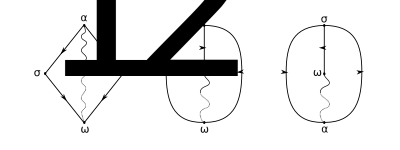
\includegraphics[width=\columnwidth]{Cells}
	\end{columns}
\end{frame}

\begin{frame}
	\frametitle{Теоретическая часть}
	\framesubtitle{Часть 6}
	Пусть $A$ - ячейка из $M'$, $\alpha$ и $\omega$ - источник и сток, входящие в её границу. Кривую $\tau\in A$, началом и концом которой являеются $\alpha$ и $\omega$, будем называть $t-$кривой. Через $T$ обозначим множество $t-$кривых, взятых по одной из каждой ячейки.
	\par Разобьём каждую ячейку этой кривой на 2 области, компоненты связности $M_\Delta = M' \textbackslash T$ назовём треугольными областями. В границу каждой треугольной области входят 3 периодические точки: источник, сток и седло, а также устойчивая сепаратриса, неусточивая сепаратриса и кривая $\tau$. В дальнейшем будем называть их $s-$кривой, $u-$кривой и $t-$кривой соответственно. Замыкание каждой из этих кривых будем называть стороной треугольной области. Скажем, что сторона является общей стороной для двух треугольных областей, если она принадлежит замыканиям этих треугольных областей.
\end{frame}
\begin{frame}
\frametitle{Теоретическая часть}
\framesubtitle{Часть 7}
	\begin{definition} Граф T называется трёхцветным графом, если:
		\par 1) множество рёбер графа T является объединением трёх подмножеств, каждое из которых состоит из трёх рёбер одного и того же определенного цвета (цвета рёбер из разных подмножеств не совпадают, будем обозначать эти цвета буквами s, t, u, а рёбра для краткости будем называть s-, t-, u-рёбрами);
		\par 2) каждая вершина графа T инцидентна в точности трём рёбрам различных цветов;
		\par 3) граф не содержит циклов длины 1.
	\end{definition}
\end{frame}

\begin{frame}
	\frametitle{Теоретическая часть}
	\framesubtitle{Часть 8}
	\begin{definition}
		Простой цикл трёхцветного графа T назовём двухцветным su-, tu- или st-циклом, если он содержит рёбра в точности двух цветов s и u, t и u, s и t соответственно.
	\end{definition}
	Непосредственно из определения трёхцветного графа следует, что длина любого двухцветного цикла является чётным числом (так как цвета рёбер строго чередуются), а отношение на множестве вершин, состоящее в принадлежности двухцветному циклу определённого типа, является отношением эквивалентности, то есть каждая отдельно взятая вершина лежит в точности в одном  $su-$, одном $tu-$ и одном $st-$цикле.
\end{frame}

\begin{frame}
	\frametitle{Теоретическая часть}
	\framesubtitle{Часть 9}
	\begin{definition}
		Построим трёхцветный граф $T_f$, соответствующий диффеоморфизму $f \in G$, следующим образом:
		\par 1) вершины графа $T_f$ взаимно однозначно соответствуют треугольным областям множества $\Delta$;
		\par 2) две вершины графа инцидентны ребру цвета s, t, u, если соответствующие этим вершинам треугольные области имеют общую s-, t- или u-кривую .
	\end{definition}
	Отметим, что построенный граф $T_f$ полностью удовлетворяет определению трёхцветного графа.
\end{frame}

\begin{frame}
	\frametitle{Теоретическая часть}
	\framesubtitle{Часть 10}
	\begin{definition}
		Трёхцветный граф (T,P) назовём допустимым, если он обладает следующими свойствами:
		\par 1) граф T связен;
		\par 2) длина любого su-цикла графа T равна 4;
		\par 3) автоморфизм P является периодическим.
	\end{definition}
	Отметим, что трёхцветный граф, построенный по градиентно-подобному каскаду на поверхности, является допустимым. Следующие теоремы сформулированы для трёхцветных графов, оснащённых автоморфизмом, однако, во избежание излишей громоздкости теоретической части, данная часть повествования была опущена в курсовой работе.
\end{frame}

\begin{frame}
	\frametitle{Теоретическая часть}
	\framesubtitle{Часть 11}
	\begin{theorem}
		Для того чтобы диффеоморфизмы f, f' из класса G были топологически сопряжены, необходимо и достаточно, чтобы их графы ($T_f, P_f$) и ($T_{f'}, P_{f'}$) были изоморфны.
	\end{theorem}
	\begin{theorem}
		Пусть (T,P) - допустимый трёхцветный граф. Тогда существует диффеоморфизм $f:M^2 \rightarrow M^2$ из класса G, граф ($T_f, P_f$) которого изоморфен графу (T,P). При этом:
		\par 1) эйлерова характеристика поверхности $M^2$ вычисляется по формуле $X(M^2) = v_0 - v_1 + v_2$, где $v_0, v_1, v_2$ - число всех tu-, su-, st-циклов графа T соответственно;
		\par 2) поверхность $M^2$ ориентируема тогда и только тогда, когда все циклы графа T имеют чётную длину.
	\end{theorem}
\end{frame}

\begin{frame}
	\frametitle{Алгоритмическая часть}
	\framesubtitle{Часть 1}
	Программа состоит из 2 частей: алгоритмической и графической, каждая из частей запускается отдельно и независимо друг от друга. Изначально запускается алгоритмическая часть на языке C++, туда вводится корректный трёхцветный граф, программа его обрабатывает и выдаёт в отдельном файле координаты сепаратрис. Далее запускается графическая часть программы, написанная на языке Python. Она считывает координаты из файла и генерирует по заданным координатам конца и начала сепаратрис 3D-изображение, а затем, после рендеринга в библиотеке Manim, показывает её пользователю.
\end{frame}

\begin{frame}
	\frametitle{Алгоритмическая часть}
	\framesubtitle{Часть 2}
	На языке C++ написаны следующие функции (краткий список):
	\begin{itemize}
		\item Проверка введённого трёхцветного графа на корректность
		\begin{itemize}
			\item Поиск в ширину
			\item Поиск двухцветных циклов
			\item Проверка графа на трёхцветность, неориентируемость и отсутствие петель
		\end{itemize}
		\item Проверка поверхности на ориентируемость при помощи базы циклов
		\item Генератор графов по заданной характеристике Эйлера и числу
		сёдел
		\item Поиск координат начала и конца сепаратрис для отображения на сферу
		\begin{itemize}
			\item Поиск соседних неподвижных точек
			\item Проверка сепаратрис на пересечение
		\end{itemize}
	\end{itemize}
\end{frame}

\begin{frame}
	\frametitle{База циклов}
	\framesubtitle{Часть 1}
	Для построения алгоритма, проверяющего поверхность, на которой задан градиентно-подобный каскад, по трёхцветному графу, потребуется пункт 2 теоремы 2, который гласит о том, что поверхности ориентируема тогда и только тогда, когда все циклы графа имеют чётную длину.
	\par Сделать вывод о четной длине всех циклов графа можно найдя хотя бы один цикл нечётной длины. Для нахождения такого цикла потребуется небольшой экскурс в теорию, связанную с базой циклов и алгоритмом её нахождения.
\end{frame}

\begin{frame}
	\frametitle{База циклов}
	\framesubtitle{Часть 2}
	Базой циклов неориентированного графа является такой набор циклов, путём соединения или вычитания которых могут получиться все остальные циклы. Для нахождения базы циклов необходимо построить из графа так называемое <<переплетающееся дерево>> (spanning tree), то есть просто выбрать какую-нибудь вершину за корень дерева, а потом идти по нему уже упомянутым выше алгоритмом поиска в ширину из корневой вершины, при этом вместо поиска расстояний отмечать посещённые вершины, если вершина-сосед не посещена, то ребро, связывающее текущую вершину с ней, добавлять в <<переплетающееся дерево>>, а далее, путём добавления по одному в дерево рёбер изначального графа, которые в дерево не попали, по одному найти все циклы. Эти циклы и будут составлять базу циклов в графе. Очевидно, что при вычитании или сложении циклов четной длины получится цикл чётной длины, то есть на чётность достаточно проверить всего лишь циклы из базы циклов.
\end{frame}

\begin{frame}
	\frametitle{База циклов}
	\framesubtitle{Часть 3}
	Алгоритм, находящий <<переплетающееся дерево>> и сразу проверяющий циклы базы циклов на чётную длину, реализован в функции $is \textunderscore oriented \textunderscore surface$, которая возвращает True, если поверхность ориентируема, и False, если поверхность неориентируема.
\end{frame}

\begin{frame}
	\frametitle{Тривиальный генератор трёхцветных графов}
	\framesubtitle{Часть 1}
	Для дальнейшей проверки алгоритма на корректность потребуется генерировать корректные трёхцветные графы со всевозможным количеством стоков и источников, такие, что соответствующие им градиентно-подобные каскады расположены на сфере, по заданному числу сёдел $\sigma$. Изложенную ниже генерацию можно обобщить для генерации трёхцветных графов, такие, что соответствующие им градиентно-подобные каскады расположены на ориентируемой поверхности, определяемой характеристикой Эйлера $e$.
\end{frame}

\begin{frame}
	\frametitle{Тривиальный генератор трёхцветных графов}
	\framesubtitle{Часть 2}
	Из определения 10 известно, что длина SU-циклов корректного трёхцветного графа равна 4, причём количество SU-циклов равно числу сёдел $\sigma$. Тогда расположим <<квадраты>> SU-циклов, верхнее и нижнее ребро которых имеют одинаковый цвет для всех <<квадратов>> (будем считать, что верхние и нижние ребра - s-рёбра), в ряд и будем проводить из каждой вершины рёбра цвета t. Далее будем соединять t-ребром с ближайшей вершиной ближайшего соседнего <<квадрата>> SU-цикла, кроме первых 2 и последних 2 вершин, которые соединяются между собой соответственно. Получили тривиальный пример графа с числом SU-циклов, равному $\sigma$, числом ST-циклов, равному $1$, и числом UT-циклов, равному $\sigma+1$.
\end{frame}
\begin{frame}
	\frametitle{Тривиальный генератор трёхцветных графов}
	\framesubtitle{Тривиальные графы на сфере}
	\begin{columns}
		\column{0.75\textwidth}
		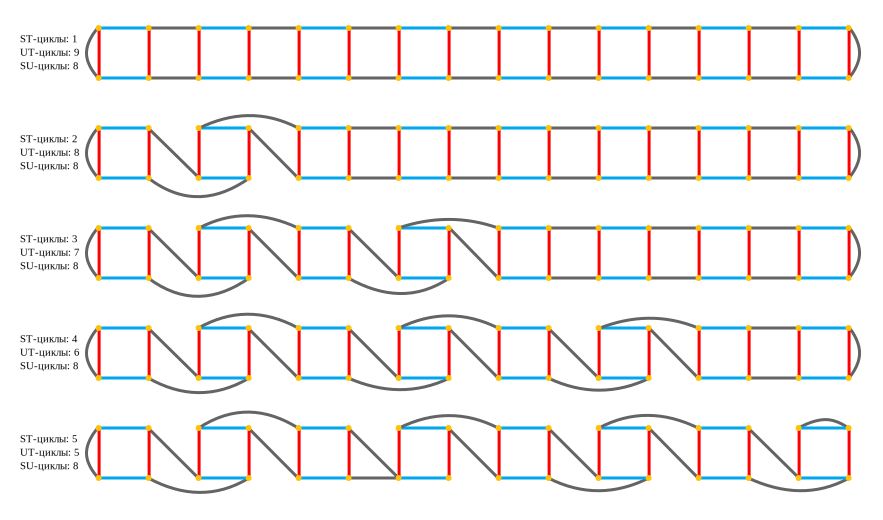
\includegraphics[width=\columnwidth]{Spheres}
	\end{columns}
\end{frame}
\begin{frame}
	\frametitle{Тривиальный генератор трёхцветных графов}
	\framesubtitle{Часть 3}
	Увеличим количество ST-циклов на 1 и уменьшим количество UT-циклов на 1. Это можно сделать из построенного выше тривиального графа при помощи переподвязок t-циклов. Переподвязывать t-циклы будем следующим способом: возьмём чётный по счёту <<квадрат>> и перекрасим s-рёбра в u-рёбра и наоборот. Одна такая переподвязка увеличивает количество ST-циклов на 1 и уменьшает количество UT-циклов на 1.
	\par Проводя такие переподвязки на чётных <<квадратах>> по одной поверх друг друга, сгенерируем циклы, для которых количество ST-циклов принимает значения (с учётом тривиального графа) $\{1,~...~, [\sigma/2]\}$, а количество UT-циклов $\{[(\sigma + 1)/2],~...~, \sigma+1\}$.
	\par Ниже приведены примеры построения трёхцветных графов при $\sigma=8$ и $e=0$ и $e=-2$ для рис. 3 и для рис. 4 соответственно.
\end{frame}
\begin{frame}
	\frametitle{Тривиальный генератор трёхцветных графов}
	\framesubtitle{Тривиальные графы на торе}
	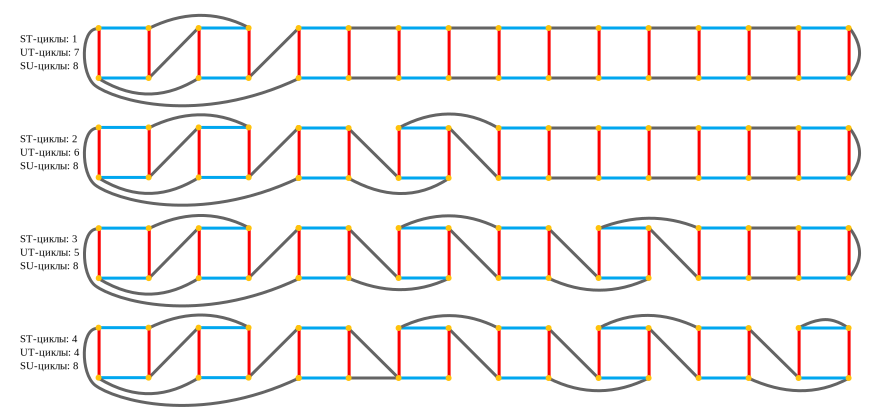
\includegraphics[width=\columnwidth]{Torus}
\end{frame}
\begin{frame}
	\frametitle{Тривиальный генератор трёхцветных графов}
	\framesubtitle{Тривиальные графы на двойном торе}
	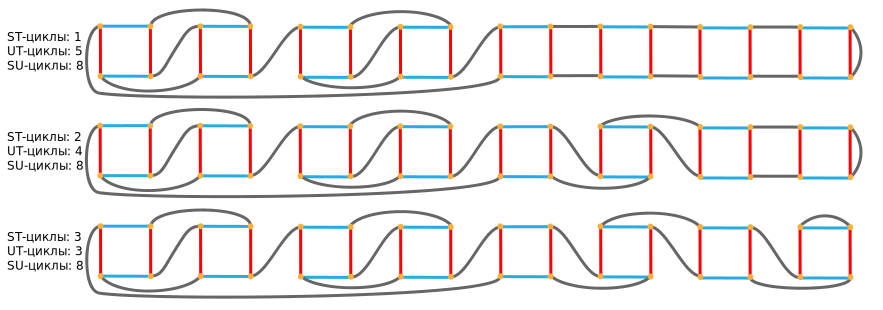
\includegraphics[width=\columnwidth]{Double Torus}
\end{frame}

\begin{frame}
	\frametitle{Алгоритмическая часть}
	\framesubtitle{Часть 3}
	Представим сферу как прямоугольник $[-90, 90]$ x $[0, 360]$, где все точки из отрезка $-90$ х $[0, 360]$ и из отрезка $90$ x $[0, 360]$ отождествлены между собой. Впоследствии при визуализации этот прямоугольник будем отображать на сферу по формуле:
	$$ \begin{cases}
		x = r * sin(\psi) * cos(\phi)\\
		x = r * sin(\psi) * sin(\phi)\\
		x = r * cos(\psi)
	\end{cases} $$ Сепаратрисы будем представлять как пары, состоящие из цвета сепаратрисы, красная или синяя, и вектора координат, содержащего $a, a0, b, b0$ и при этом заданной формулой:
	$$ \begin{cases}
		x = a * t + a_0\\
		y = b * t + b_0
	\end{cases} $$ где t $\in [0, 1]$.
\end{frame}
\begin{frame}
	\frametitle{Алгоритмическая часть}
	\framesubtitle{Представление каскада на сфере}
	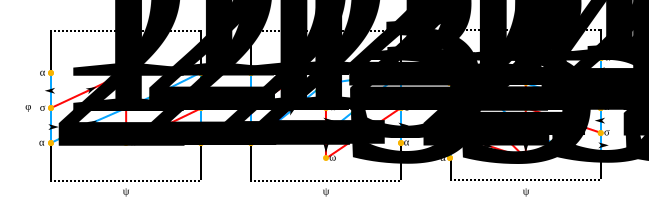
\includegraphics[width=\textwidth]{Projections.png}
\end{frame}
\begin{frame}
\frametitle{Unit-тестирование}
	Для стабильной работы программы при изменении в дальнейшем в каталоге под названием $graph \textunderscore algorithms \textunderscore unit \textunderscore test$ содержатся файлы, в которых написаны unit-тесты для различных функций. Если при изменении программа будет работать неправильно, то unit-тесты распознают аномалии.
\end{frame}
\begin{frame}
\frametitle{Графическая часть}
\framesubtitle{Часть 1}
	Графическая часть программы, написанная в файле draw.py, отвечает за генерацию 3D-изображения дискретной динамической системы на сфере.
	\par В файле определён класс DynamicalSystemSphere, который в дальнейшем будет указываться при запуске графической части.
	\par Графическая часть работает по следующему алгоритму:
	\par 1) Считывается информация о сепаратрисах, полученная в результате запуска алгоритмической части;
	\par 2) Объявляется функция $func \textunderscore sphere$, задающая параметрически поверхность сферы:
	$$ \begin{cases}
		x = r * cos(u) * sin(v) - x_0\\
		y = r * sin(u) * sin(v) - y_0\\
		z = r * cos(v) - z_0
	\end{cases} $$
	\par 3) Объявляется функция $construct$, которая отвечает непосредственно за генерацию 3D-изображения. При помощи библиотеки Manim создаются поверхность сферы и оси OX, OY и OZ. Далее каждая сепаратриса, разбитая на 3 равные части, отличающиеся по цвету: более яркий красный и синий цвет соответствуют близости к стокам и источникам соответственно, а бледные оттенки этих цветов соответствуют близости к седлу, по отдельности добавляется на поверхность сферы.
\end{frame}
\begin{frame}
	\frametitle{Графическая часть}
	\framesubtitle{Часть 2}
	Cепаратриса, заданная параметрически на прямоугольнике значениями $a, a0, b, b0$, отображается на поверхность сферы по правилу:
	$$ \begin{cases}
		x = cos(pi * (t * b + b_0) / 180) * sin(pi * (t * a + a_0) / 180)\\
		y = cos(pi * (t * b + b_0) / 180) * cos(pi * (t * a + a_0) / 180)\\
		z = sin(pi * (t * b + b_0) / 180)
	\end{cases} $$ где t принадлежит [0, 1] (причём для создания более <<говорящей>> картинки для различных оттенков сепаратрисы отрезок разбивается на 3 равные части, каждая из которых отображается независимо от остальных).
	\par Для получения объёмного и <<говорящего>> изображения объявляется полный оборот камеры вокруг сферы.
\end{frame}
\begin{frame}
\frametitle{Запуск и результат работы программы}
	Для запуска генерации 3D-изображения необходимо:
	\par 1) При помощи терминала установить библиотеку Manim на компьютер, если эта библиотека ещё не установлена.
	\par 2) Предварительно запустить алгоритмическую часть с введённым в неё корректным трёхцветным графом.
	\par 3) При помощи терминала перейти в каталог с файлом draw.py.
	\par 4) Запустить графическую часть при помощи команды:
	\par manim -pqh draw.py DynamicalSystemSphere - для генерации изображения высокого качества;
	\par manim -pql draw.py DynamicalSystemSphere - для генерации изображения низкого качества.
\end{frame}
\begin{frame}
\includegraphics[width=\columnwidth]{Example}
\end{frame}
\begin{frame}
\frametitle{Ссылка на репозиторий в Github}
	Ссылка на репозиторий: $https://github.com/dan1lka257/graphs \textunderscore and \textunderscore algorithms/tree/main$
\end{frame}

\end{document}